\section{Teilversuch 1: Bestimmung der spezifischen Wärmekapazität von Wasser}
	\subsection{Wasserwert des Kalorimeters}
	  	Als Messungen haben wir:
	  	\begin{equation*}
	  		\begin{tabu}{lll}
	  			\text{Temperaturen} && \\
	  			\toprule
	  			\text{Kalt } & (\theta_1) & \SI{24.0(1)}{\celsius} \\
	  			\text{Warm } & (\theta_2) & \SI{74.2(1)}{\celsius} \\
	  			\text{Mischung } & (\theta_m) & \SI{36.5(1)}{\celsius} \\
	  			\bottomrule
	  		\end{tabu}
	  	\end{equation*}
	  	\begin{equation*}
	  		\begin{tabu}{lll|l}
	  			\text{Gewichten} \\
	  			\toprule
	  			& M_{0}/\si{\gram} & M_1/\si{\gram} & M_i/\si{\gram}\\
	  			\midrule
	  			\text{Kalt }(M_k) & \num{908.60(13)} & \num{306.92(3)} & \num{601.68(14)}\\
	  			\text{Warm }(M_w) & \num{509.03(3)} & \num{294.31(3)}  & \num{214.72(4)}\\
	  			\bottomrule
	  		\end{tabu}
	  	\end{equation*}
	  	wobei $M_0$ das Gewicht der Wasser plus Gefäß und $M_1$ das Gewicht der Gefäß mit ggf. übriges Wasser ist. Die jeweiligen Massen von Wasser $M_i$ sind gegeben durch $M_i = M_1 - M_0$, mit dem entsprechenden Fehler:
	  	\begin{align}
	  		\Delta M_i = \sqrt{(\Delta M_0)^2 + (\Delta M_1)^2}
	  	\end{align}
	  	Aus der Anleitung ist der Wasserwert des Kalorimeters gegeben durch:
	  	\begin{equation}
	  		m_w^* = \frac{M_w(\theta_2 - \theta_m)}{(\theta_m - \theta_1)} - M_k
	  	\end{equation}
	  	und der Fehler:
	  	\begin{align}
	  		\Delta (\theta_2 - \theta_m) &= \addquad{\theta_1, \theta_m} = \sqrt{2} \Delta\theta = \Delta (\theta_m - \theta_1)\\\
	  		(\Delta m_w^*)^2 &=  \left(\frac{M_w(\theta_2 - \theta_m)}{(\theta_m - \theta_1)} 
	  		\relquad{(\theta_2 - \theta_m), (\theta_m - \theta_1), M_w}\right)^2 \notag \\
	  		&\phantom{=}+ \left(\Delta M_k\right)^2 \\
	  		&= \left(\frac{M_w(\theta_2 - \theta_m)}{(\theta_m - \theta_1)}\sqrt{2(\Delta\theta)^2\left(\frac{1}{(\theta_2 - \theta_m)^2} + \frac{1}{(\theta_m - \theta_1)^2}\right) + \left(\frac{\Delta M_w}{M_w}\right)^2}\right)^2 \notag \\
	  		&\phantom{=}+ \left(\Delta M_k\right)^2 \\
	  		&= \left(\frac{M_w(\theta_2 - \theta_m)}{(\theta_m - \theta_1)}\right)^2\cdot\left({2(\Delta\theta)^2\left(\frac{1}{(\theta_2 - \theta_m)^2} + \frac{1}{(\theta_m - \theta_1)^2}\right) + \left(\frac{\Delta M_w}{M_w}\right)^2}\right) \notag \\
	  		&\phantom{=}+ \left(\Delta M_k\right)^2 
	  	\end{align}
	  	Wir substituieren die Werten:
	  	\begin{align*}
	  		m_w^* &= \frac{(\SI{214.72}{\gram})(\SI{74.2}{\celsius} - \SI{36.5}{\celsius})}{(\SI{36.5}{\celsius} - \SI{24.0}{\celsius})} - \SI{601.68}{\gram} \\
	  		&= \frac{(\SI{214.72}{\gram})(\SI{37.7}{\celsius})}{(\SI{12.5}{\celsius})} - \SI{601.68}{\gram}\\
	  		&= \SI{647.59552}{\gram} - \SI{601.68}{\gram}\\
	  		&= \SI{45.91552}{\gram}\\
	  		(\Delta m_w^*)^2 &= \left(\SI{647.59552}{\gram}\right)^2\cdot\left({2(\SI{0.1}{\celsius})^2\left(\frac{1}{(\SI{37.7}{\celsius})^2} + \frac{1}{(\SI{12.5}{\celsius})^2}\right) + \left(\frac{\SI{0.04}{\gram}}{\SI{214.72}{\gram}}\right)^2}\right) \notag \\
	  		&\phantom{=}+ \left(\SI{0.14}{\gram}\right)^2  \\
	  		\Delta m_w^* &= \SI{29.8919}{\gram} \sigfig{6}
	  	\end{align*}
	  	Somit ist $m_w^* = \SI{50(30)}{\gram}$. Der im Kapitel 1.4 gegebene Literaturwert $m_w^* = \SI{80}{\gram}$ liegt im Fehlerintervall des experimental bestimmten Wert, also stimmt die beide Werten miteinander überein. Es ist hier zu bemerken, dass der experimental bestimmte Wert eine sehr große Unsicherheit hat. 

	  	%Der experimental bestimmte Wert hat aber eine sehr große Unsicherheit, also benutzen wir den Literaturwert für alle andere Berechnungen.

	\newpage
	\subsection{Spezifische Wärmekapazität von Wasser}
		Fehler bei Messung der Zeit $\Delta t = \SI{0.2}{\second}$ \\
		Fehler bei Messung der Temperatur $\Delta x = \SI{0.3}{\celsius}$ 
		\begin{equation*}
			\begin{tabu}{l *{8}{l}}
				\multicolumn{9}{l}{\text{Messreihe}} \\
				\toprule
				t/\si{\minute} & 0 & 60 & 120 & 180 & 240 & 300 & 360 & 420 \\
				\midrule
				\theta/\si{\celsius} & 25,6 & 26,5 & 26,7 & 27,0 & 27,6 & 28,1 & 28,6 & 29,1  \\
				\bottomrule
				\toprule
				t/\si{\minute} & 480 & 540 & 600 & 660 & 720 & 780 & 840 & 900 \\
				\midrule
				\theta/\si{\celsius} & 29,5 & 30,2 & 30,8 & 31,2 & 31,6 & 32,0 & 32,9 & 33,1 \\
				\bottomrule
			\end{tabu}
		\end{equation*}
		Die Daten wurden dann mit \gnuplot{} geplottet und es wurde eine Kurvenanpassung zur $\theta = bt + c$ durchgeführt.
		\begin{figure}[H]
			\centering
			% GNUPLOT: LaTeX picture with Postscript
\begingroup
  \makeatletter
  \providecommand\color[2][]{%
    \GenericError{(gnuplot) \space\space\space\@spaces}{%
      Package color not loaded in conjunction with
      terminal option `colourtext'%
    }{See the gnuplot documentation for explanation.%
    }{Either use 'blacktext' in gnuplot or load the package
      color.sty in LaTeX.}%
    \renewcommand\color[2][]{}%
  }%
  \providecommand\includegraphics[2][]{%
    \GenericError{(gnuplot) \space\space\space\@spaces}{%
      Package graphicx or graphics not loaded%
    }{See the gnuplot documentation for explanation.%
    }{The gnuplot epslatex terminal needs graphicx.sty or graphics.sty.}%
    \renewcommand\includegraphics[2][]{}%
  }%
  \providecommand\rotatebox[2]{#2}%
  \@ifundefined{ifGPcolor}{%
    \newif\ifGPcolor
    \GPcolortrue
  }{}%
  \@ifundefined{ifGPblacktext}{%
    \newif\ifGPblacktext
    \GPblacktexttrue
  }{}%
  % define a \g@addto@macro without @ in the name:
  \let\gplgaddtomacro\g@addto@macro
  % define empty templates for all commands taking text:
  \gdef\gplbacktext{}%
  \gdef\gplfronttext{}%
  \makeatother
  \ifGPblacktext
    % no textcolor at all
    \def\colorrgb#1{}%
    \def\colorgray#1{}%
  \else
    % gray or color?
    \ifGPcolor
      \def\colorrgb#1{\color[rgb]{#1}}%
      \def\colorgray#1{\color[gray]{#1}}%
      \expandafter\def\csname LTw\endcsname{\color{white}}%
      \expandafter\def\csname LTb\endcsname{\color{black}}%
      \expandafter\def\csname LTa\endcsname{\color{black}}%
      \expandafter\def\csname LT0\endcsname{\color[rgb]{1,0,0}}%
      \expandafter\def\csname LT1\endcsname{\color[rgb]{0,1,0}}%
      \expandafter\def\csname LT2\endcsname{\color[rgb]{0,0,1}}%
      \expandafter\def\csname LT3\endcsname{\color[rgb]{1,0,1}}%
      \expandafter\def\csname LT4\endcsname{\color[rgb]{0,1,1}}%
      \expandafter\def\csname LT5\endcsname{\color[rgb]{1,1,0}}%
      \expandafter\def\csname LT6\endcsname{\color[rgb]{0,0,0}}%
      \expandafter\def\csname LT7\endcsname{\color[rgb]{1,0.3,0}}%
      \expandafter\def\csname LT8\endcsname{\color[rgb]{0.5,0.5,0.5}}%
    \else
      % gray
      \def\colorrgb#1{\color{black}}%
      \def\colorgray#1{\color[gray]{#1}}%
      \expandafter\def\csname LTw\endcsname{\color{white}}%
      \expandafter\def\csname LTb\endcsname{\color{black}}%
      \expandafter\def\csname LTa\endcsname{\color{black}}%
      \expandafter\def\csname LT0\endcsname{\color{black}}%
      \expandafter\def\csname LT1\endcsname{\color{black}}%
      \expandafter\def\csname LT2\endcsname{\color{black}}%
      \expandafter\def\csname LT3\endcsname{\color{black}}%
      \expandafter\def\csname LT4\endcsname{\color{black}}%
      \expandafter\def\csname LT5\endcsname{\color{black}}%
      \expandafter\def\csname LT6\endcsname{\color{black}}%
      \expandafter\def\csname LT7\endcsname{\color{black}}%
      \expandafter\def\csname LT8\endcsname{\color{black}}%
    \fi
  \fi
    \setlength{\unitlength}{0.0500bp}%
    \ifx\gptboxheight\undefined%
      \newlength{\gptboxheight}%
      \newlength{\gptboxwidth}%
      \newsavebox{\gptboxtext}%
    \fi%
    \setlength{\fboxrule}{0.5pt}%
    \setlength{\fboxsep}{1pt}%
\begin{picture}(8640.00,5760.00)%
    \gplgaddtomacro\gplbacktext{%
      \csname LTb\endcsname%%
      \put(682,704){\makebox(0,0)[r]{\strut{}$25$}}%
      \put(682,1192){\makebox(0,0)[r]{\strut{}$26$}}%
      \put(682,1681){\makebox(0,0)[r]{\strut{}$27$}}%
      \put(682,2169){\makebox(0,0)[r]{\strut{}$28$}}%
      \put(682,2657){\makebox(0,0)[r]{\strut{}$29$}}%
      \put(682,3146){\makebox(0,0)[r]{\strut{}$30$}}%
      \put(682,3634){\makebox(0,0)[r]{\strut{}$31$}}%
      \put(682,4122){\makebox(0,0)[r]{\strut{}$32$}}%
      \put(682,4611){\makebox(0,0)[r]{\strut{}$33$}}%
      \put(682,5099){\makebox(0,0)[r]{\strut{}$34$}}%
      \put(814,484){\makebox(0,0){\strut{}$-100$}}%
      \put(1489,484){\makebox(0,0){\strut{}$0$}}%
      \put(2165,484){\makebox(0,0){\strut{}$100$}}%
      \put(2840,484){\makebox(0,0){\strut{}$200$}}%
      \put(3515,484){\makebox(0,0){\strut{}$300$}}%
      \put(4191,484){\makebox(0,0){\strut{}$400$}}%
      \put(4866,484){\makebox(0,0){\strut{}$500$}}%
      \put(5542,484){\makebox(0,0){\strut{}$600$}}%
      \put(6217,484){\makebox(0,0){\strut{}$700$}}%
      \put(6892,484){\makebox(0,0){\strut{}$800$}}%
      \put(7568,484){\makebox(0,0){\strut{}$900$}}%
      \put(8243,484){\makebox(0,0){\strut{}$1000$}}%
    }%
    \gplgaddtomacro\gplfronttext{%
      \csname LTb\endcsname%%
      \put(209,2901){\rotatebox{-270}{\makebox(0,0){\strut{}Temperatur $\theta$ ($\si{\celsius}$)}}}%
      \put(4528,154){\makebox(0,0){\strut{}Zeit $t$ ($\si{\second}$)}}%
      \csname LTb\endcsname%%
      \put(946,4893){\makebox(0,0)[l]{\strut{}$0,00832t + 25,66397$}}%
      \csname LTb\endcsname%%
      \put(946,4607){\makebox(0,0)[l]{\strut{}Messpunkte}}%
      \csname LTb\endcsname%%
      \put(4528,5429){\makebox(0,0){\strut{}Erwärmung von Wasser im Kalorimeter}}%
    }%
    \gplbacktext
    \put(0,0){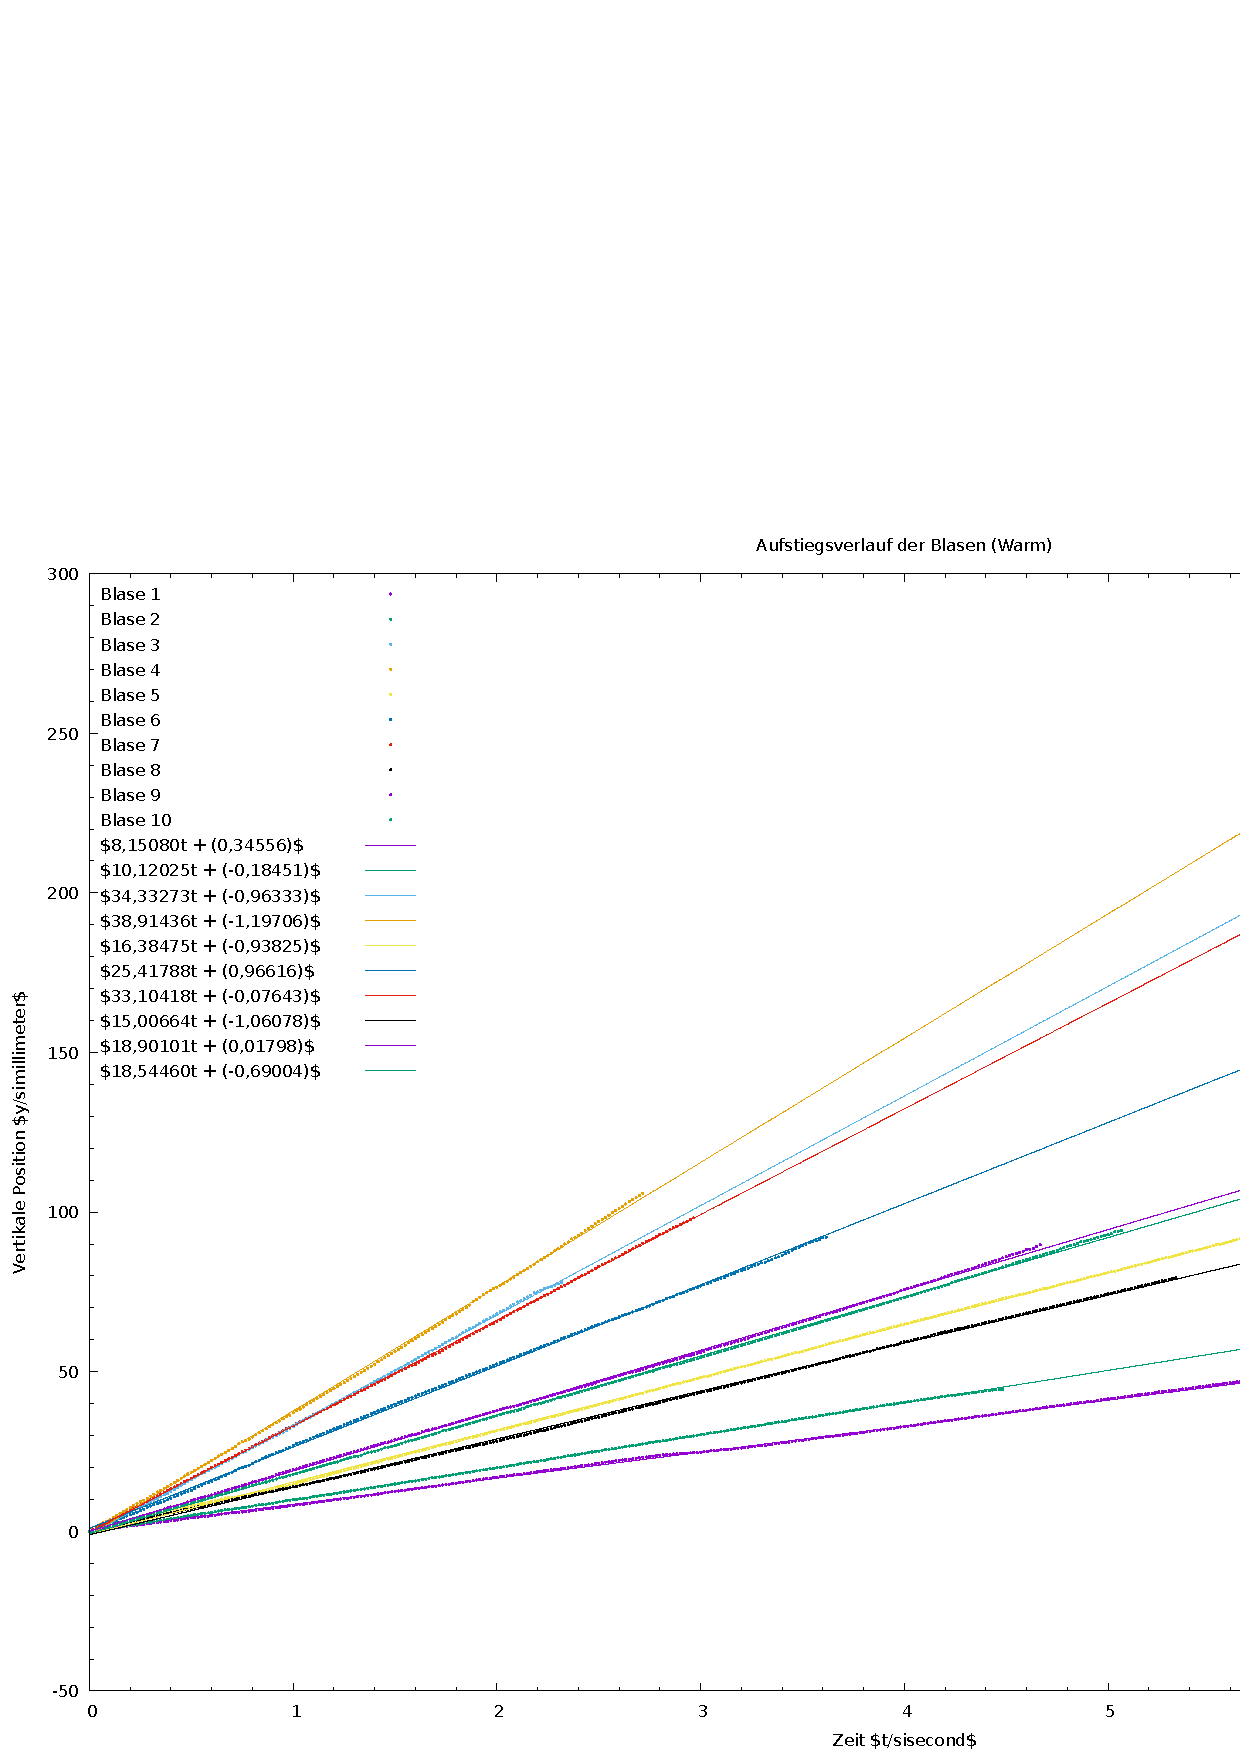
\includegraphics[width={432.00bp},height={288.00bp}]{tv1-plot}}%
    \gplfronttext
  \end{picture}%
\endgroup

			\caption{\centering Temperaturverlauf bei der Erwärmung von Wasser im Kalorimeter \captionbr $\chi^2_{\text{red}} = \num{0.237306} \implies$ Gute Anpassung}
			\label{fig:tvone-plot}
			\vspace{-1em}
		\end{figure}
		Als Endergebnis erhalten wir:
		\begin{equation*}
			\begin{tabu}{ll}
				\toprule
				b & \SI{8.3162(1321)e-3}{\celsius\per\second} \\
				c & \SI{25.664(70)}{\celsius} \\
				\bottomrule
			\end{tabu}
		\end{equation*}
		Gerundet haben wir $b = \SI{8.32(14)e-3}{\kelvin\per\second}$, da eine $\SI{1}{\kelvin}$ Änderung die gleiche wie eine $\SI{1}{\celsius}$ Änderung ist. 

		Aus der Anleitung gilt:
		\begin{align}
			Q = mC_S \Delta \theta && \Leftrightarrow && IV\Delta t = mC_S \Delta \theta && \Leftrightarrow && \frac{\Delta \theta}{\Delta t} = \frac{IV}{mC_S} 
		\end{align}
		Also ist die Steigung $\displaystyle b = \frac{IV}{mC_S}$ und es gilt:
		\begin{align}
			C_S = \frac{IV}{mb} = \frac{IV}{(m_w + m_w^*)\,b} = \frac{IV}{((m_\text{w+g} - m_\text{g}) + m_w^*)\,b}
		\end{align}
		Da wir nur die Unsicherheiten der Geradensteigung und die Unsicherheit des Wasserwertes berücksichtigen müssen, vernachlässigen wir die Unsicherheiten bei $m_\text{w+g}$, $m_\text{g}$, $I$ und $V$. Der Fehler ist somit gegeben durch:
		\begin{align*}
			C_S = \gausserror{C_S}{m_w^*,b}
		\end{align*}
		mit
		\begin{align*}
			\pdv{C_S}{m_w^*} = - \frac{IV}{b\,(m_\text{w+g} - m_\text{g} + m_w^*)^2} && \pdv{C_S}{b} = - \frac{IV}{b^2\,(m_\text{w+g} - m_\text{g} + m_w^*)}
		\end{align*}
		Es gilt somit:
		\begin{align*}
			\Delta C_S = \sqrt{\left(\frac{IV \Delta m_w^*}{b\,(m_\text{w+g} - m_\text{g} + m_w^*)^2}\right)^2 + \left(\frac{IV \Delta b}{b^2\,(m_\text{w+g} - m_\text{g} + m_w^*)}\right)^2} 
		\end{align*}
		Wir haben als Messwerten:
		\begin{equation*}
			\begin{tabu}{lll}
				\toprule
				\text{Variable} & \text{Wert} & \text{Bedeutung}\\
				\midrule 
				V & \SI{21.50(21)}{\volt} & \text{Spannung am Heizungselement}\\
				I & \SI{1.6(6)}{\ampere} & \text{Strom am Heizungselement}\\
				m_\text{w+g} & \SI{903.20(13)}{\gram} & \text{Masse der Wasser und Gefäß} \\
				m_\text{g} & \SI{306.83(3)}{\gram} & \text{Masse des leeren Gefäß} \\
				m_w^* & \SI{50(30)}{\gram} & \text{Wasserwert des Kalorimeters} \\
				b & \SI{8.32(14)e-3}{\kelvin\per\second} & \text{Erhaltene Steigung} \\
				\bottomrule
			\end{tabu}
		\end{equation*}
		Damit:
		\begin{align*}
			C_S &= \frac{(\SI{1.6}{\ampere})(\SI{21.50}{\volt})}{(\SI{903.20}{\gram} - \SI{306.83}{\gram} + \SI{50}{\gram})\,(\SI{8.32e-3}{\kelvin\per\second})} \\
			&= \SI{6.39667}{\joule\per\gram\per\kelvin} \\
			\Delta C_S^2 &= \left(\frac{(\SI{1.6}{\ampere})(\SI{21.50}{\volt}) (\SI{30}{\gram})}{(\SI{8.32e-3}{\kelvin\per\second})\,(\SI{903.20}{\gram} - \SI{306.83}{\gram} + \SI{50}{\gram})^2}\right)^2 \\
			&\phantom{=}+ \left(\frac{(\SI{1.6}{\ampere})(\SI{21.50}{\volt})(\SI{0.14e-3}{\kelvin\per\second})}{(\SI{8.32e-3}{\kelvin\per\second})^2\,(\SI{903.20}{\gram} - \SI{306.83}{\gram} + \SI{50}{\gram})}\right)^2 \\
		\Delta C_S &= \SI{0.316471}{\joule\per\gram\per\kelvin}
		\end{align*}
		Somit erhalten wir $C_S = \SI{6.4(4)}{\joule\per\gram\per\kelvin}$.

		Für den Literaturwert benutzen wir den Mittelwert von den Temperaturen und verwenden die Wärme\-kapazität bei diesem Temperatur. Also $\sum_i \theta_i \si{\celsius} = \SI{29.406}{\celsius} \approx \SI{30}{\celsius}$. Der Literaturwert von der Wärmekapazität des Wassers lautet $C_{S\text{ (lit)}} = \SI{4.1801}{\joule\per\gram\per\kelvin}$ bei \SI{30}{\celsius} \footnote{\url{www.engineeringtoolbox.com/specific-heat-capacity-water-d_660.html}}.

		Folglich unterscheiden sich die Werten signifikant voneinander. 

		Dieser Unterschied kann vielleicht darauf zurückgeführt werden, dass die tatsächliche Unsicherheiten von der Messung der Spannung nicht berücksichtigt würden. Während der Messungen wurde beobachtet, dass die Spannung sich im Verlauf des Experiements deutlich schwingt. Somit könnte die tatsächliche Unsicherheit bei der Messung deutlich größer sein als die, die der Hersteller ermittelt hat. Das hat vermütlich zu einer geringer Unsicherheit bei $C_S$ geführt. 

		Weiterhin ist das Heizungselement höchstwahrscheinlich nicht 100\% effizient, also könnte die berechnete Leistung $P=IV$ viel größer als die tatsächliche Leistung sein, was zu einem größeren $C_S$ liefern würde. 
